% Delay chain using DFFs
% Original: "D flip-flops (DFFs) and shift register" by Martin Scharrer
% (http://www.texample.net/tikz/examples/d-flip-flops-and-shift-register/)
% Modified: Anders Østevik

%\documentclass[a4paper, landscape]{article}
\documentclass[main.tex]{subfiles}

%\usepackage{pgf,tikz}
\usetikzlibrary{calc,arrows}
\usetikzlibrary{shapes.geometric}
%\usepackage{amsmath}
%\usepackage[left=1cm,right=1cm]{geometry}
%\pagestyle{empty}

\makeatletter

% Data Flip Flip (DFF) shape
\pgfdeclareshape{dff}{
  % The 'minimum width' and 'minimum height' keys, not the content, determine
  % the size
  \savedanchor\northeast{%
    \pgfmathsetlength\pgf@x{\pgfshapeminwidth}%
    \pgfmathsetlength\pgf@y{\pgfshapeminheight}%
    \pgf@x=0.4\pgf@x
    \pgf@y=0.4\pgf@y
  }
  % This is redundant, but makes some things easier:
  \savedanchor\southwest{%
    \pgfmathsetlength\pgf@x{\pgfshapeminwidth}%
    \pgfmathsetlength\pgf@y{\pgfshapeminheight}%
    \pgf@x=-0.4\pgf@x
    \pgf@y=-0.4\pgf@y
  }
  % Inherit from rectangle
  \inheritanchorborder[from=rectangle]

  % Define same anchor a normal rectangle has
  \anchor{center}{\pgfpointorigin}
  \anchor{north}{\northeast \pgf@x=0pt}
  \anchor{east}{\northeast \pgf@y=0pt}
  \anchor{south}{\southwest \pgf@x=0pt}
  \anchor{west}{\southwest \pgf@y=0pt}
  \anchor{north east}{\northeast}
  \anchor{north west}{\northeast \pgf@x=-\pgf@x}
  \anchor{south west}{\southwest}
  \anchor{south east}{\southwest \pgf@x=-\pgf@x}
  \anchor{text}{
    \pgfpointorigin
    \advance\pgf@x by -.5\wd\pgfnodeparttextbox%
    \advance\pgf@y by -.5\ht\pgfnodeparttextbox%
    \advance\pgf@y by +.5\dp\pgfnodeparttextbox%
  }

  % Define anchors for signal ports
  \anchor{D}{
    \pgf@process{\northeast}%
    \pgf@x=-1\pgf@x%
    \pgf@y=.5\pgf@y%
  }
  \anchor{CLK}{
    \pgf@process{\northeast}%
    \pgf@x=-1\pgf@x%
    \pgf@y=-.66666\pgf@y%
  }
  \anchor{Q}{
    \pgf@process{\northeast}%
    \pgf@y=.5\pgf@y%
  }
  % Draw the rectangle box and the port labels
  \backgroundpath{
    % Rectangle box
    \pgfpathrectanglecorners{\southwest}{\northeast}
    % Angle (>) for clock input
    \pgf@anchor@dff@CLK
    \pgf@xa=\pgf@x \pgf@ya=\pgf@y
    \pgf@xb=\pgf@x \pgf@yb=\pgf@y
    \pgf@xc=\pgf@x \pgf@yc=\pgf@y
    \pgfmathsetlength\pgf@x{1.6ex} % size depends on font size
    \advance\pgf@ya by \pgf@x
    \advance\pgf@xb by \pgf@x
    \advance\pgf@yc by -\pgf@x
    \pgfpathmoveto{\pgfpoint{\pgf@xa}{\pgf@ya}}
    \pgfpathlineto{\pgfpoint{\pgf@xb}{\pgf@yb}}
    \pgfpathlineto{\pgfpoint{\pgf@xc}{\pgf@yc}}
    \pgfclosepath

    % Draw port labels
    \begingroup
    \tikzset{flip flop/port labels} % Use font from this style
    \tikz@textfont

    \pgf@anchor@dff@D
    \pgftext[left,base,at={\pgfpoint{\pgf@x}{\pgf@y}},x=\pgfshapeinnerxsep]{\raisebox{-0.75ex}{D}}

    \pgf@anchor@dff@Q
    \pgftext[right,base,at={\pgfpoint{\pgf@x}{\pgf@y}},x=-\pgfshapeinnerxsep]{\raisebox{-.75ex}{Q}}

    \endgroup
  }
}

% Key to add font macros to the current font
\tikzset{add font/.code={\expandafter\def\expandafter\tikz@textfont\expandafter{\tikz@textfont#1}}} 

% Define default style for this node
\tikzset{flip flop/port labels/.style={font=\sffamily\scriptsize}}
\tikzset{every dff node/.style={draw,minimum width=2cm,minimum 
height=2.828427125cm,very thick,inner sep=1mm,outer sep=0pt,cap=round,add 
font=\sffamily}}

\tikzset{
  multiplexer/.style={
    draw,
    trapezium,
    ultra thick,
    shape border uses incircle, 
    shape border rotate=270,
    minimum size=38pt
  }  
}

\begin{document}

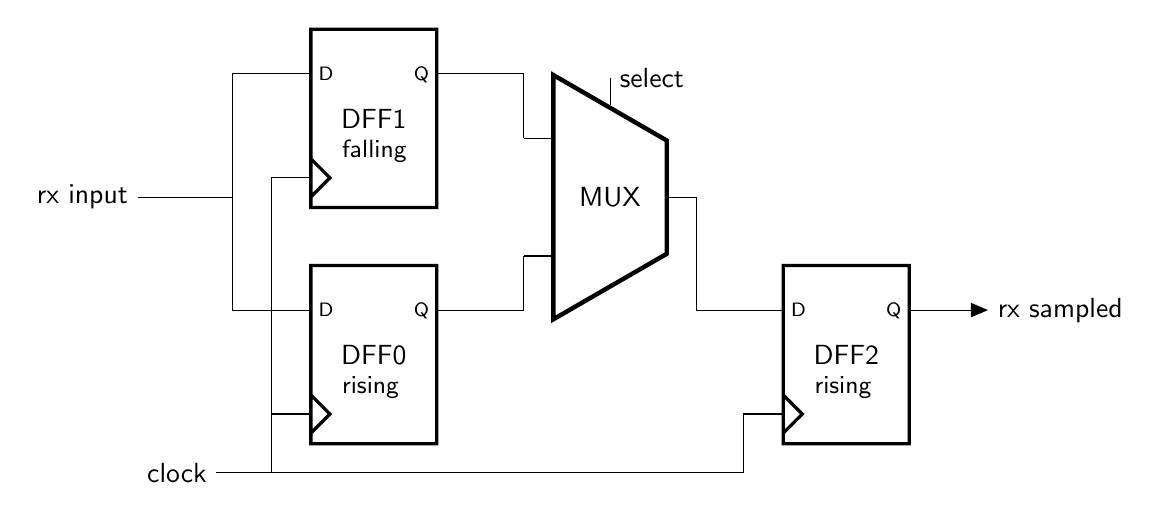
\begin{tikzpicture}[font=\sffamily,>=triangle 45]
  \def\N{1}  % Number of Flip-Flops minus one

  % Place FFs
  \foreach \m in {0,...,\N}
    \node [shape=dff] (DFF\m) at ($ 3*(0,\m) $) {DFF\m};

    \node [shape=dff] (DFF2) at ($ (6,0) $) {DFF2};

  \node[multiplexer]
    (mul) at (3,2) {MUX};
  \draw (mul.top side) --++(10pt,0); 
  \draw (mul.south west) --++(-10pt,0); 
  \draw (mul.north west) --++(-10pt,0);
  %\draw (mul.north) --++(0,10pt); 

  % Connect FFs (Q1 with D1, etc.)
  % \def\p{0}  % Used to save the previous number
  % \foreach \m in {1,...,\N} { % Note that it starts with 1, not 0
  %   \draw [->] (DFF\p.Q) -- (DFF\m.D);
  %   \global\let\p\m
  % }

  \draw [-] (DFF0.Q) -| ($(mul.south west) + (-10pt,0)$);
  \draw [-] (DFF1.Q) -| ($(mul.north west) + (-10pt,0)$);
  \draw [-] (DFF2.D) -| ($(mul.top side) + (10pt,0)$);
  % Connect and label data in- and output port
  %\draw [<-] (DFF0.D) -- +(-1,0) node [anchor=east] {input} ;

  \draw [->] (DFF2.Q) -- +(1,0) node [anchor=west] {rx sampled};

  \draw [-] (mul.north) -- +(0,10pt) node [anchor=west] {select};

  \draw [] (DFF0) +(-15pt,-12pt) node [anchor=west] {\small rising};
  \draw [] (DFF1) +(-15pt,-12pt) node [anchor=west] {\small falling};
  \draw [] (DFF2) +(-15pt,-12pt) node [anchor=west] {\small rising};


  %\node[draw,align=left] at (3,0) {some text\\ spanning three lines\\ with manual line breaks};


  % Input port label
    \path (DFF0) +(-3cm,2cm) coordinate (temp1)
    node [anchor=east] {rx input};
  \foreach \m in {0,...,\N}
    \draw [-] (temp1) -| ($ (DFF\m.D) + (-1cm,0) $) --(DFF\m.D);

  % Clock port label
  \path (DFF0) +(-2cm,-1.5cm) coordinate (temp)
    node [anchor=east] {clock};
  \foreach \m in {0,...,\N}
    \draw [-] (temp) -| ($ (DFF\m.CLK) + (-5mm,0) $) --(DFF\m.CLK);

    \draw [-] (temp) -| ($ (DFF2.CLK) + (-5mm,0) $) --(DFF2.CLK);


\end{tikzpicture}

\end{document}